\section{引入维数的想法}\label{sec:motivation-for-dimension}

维数是一个人人都很熟悉的概念. 例如, 我们大多数人大概从小就明白, 自己生活在一个三维世界里. 我们对这三个维度的理解是, 我们有三个基本的移动方向: 前后, 左右和上下. 当然, 方向并不只有这三种, 但任何其他方向都是这三种方向的组合.

\BookPairedFigure
  {对我们许多人来说, 线性代数是第一次学到维数的精确定义的数学学科. 这一定义自然体现了上一段提到的\textquotedbl{}基本\textquotedbl{}和\textquotedbl{}组合\textquotedbl{}两个概念. 回忆一下, 若域 $K$ 上的向量空间 $V$ 有一组含 $n$ 个向量的基, 就称其维数为 $n$. 重要的是, 必须检查 $V$ 的任何两组基都有相同数目的向量, 这样才能保证这一定义是良定义的. 可以把基向量看成在 $V$ 中移动的基本方向.}
  {\phantomsection\label{fig:dimension-standard-basis}%
   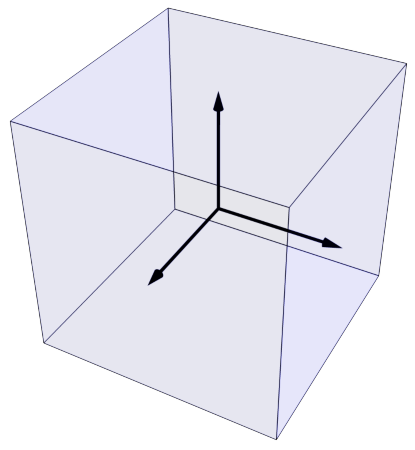
\includegraphics[width=\linewidth]{figures/dimension-standard-basis.png}}
\noindent\hyperref[fig:dimension-standard-basis]{上图}画出了 $\mathbb{R}^{3}$ 的三个标准基向量. 在 $\mathbb{R}^{3}$ 中移动的任意方向, 都可以唯一表示成这三个向量的线性组合.

\BookPairedNoteLeft
  {维数衡量在一个集合中移动的自由度, 这个直观想法将指导我们给出代数几何中的维数定义. 下面用一个熟悉的非线性例子进一步说明.}
  {注意域 $K$ 对向量空间维数的重要作用: 通常的平面作为 $\mathbb{R}$-向量空间是二维的, 但作为 $\mathbb{C}$-向量空间只有一维.}

\begin{Example}{球面的维数}\leavevmode\label{ex:dimension-of-the-sphere}
考虑球面 $X=\mathcal{V}(x^{2}+y^{2}+z^{2}-1)\subseteq\mathbb{A}^{3}$. 在实数域上, 这就是熟悉的单位球面. 甚至可以把单位球面想象成地球表面的模型.

\BookPairedFigure
  {我们自然会认为地球表面是二维的, 因为在任何位置, 我们都有两个基本的移动方向. 当不在两极时, 我们称这两个方向为南北方向和东西方向. 但是, 如何用代数精确刻画日常经验中这两个维度的自由度?}
  {\phantomsection\label{fig:dimension-blue-marble}%
   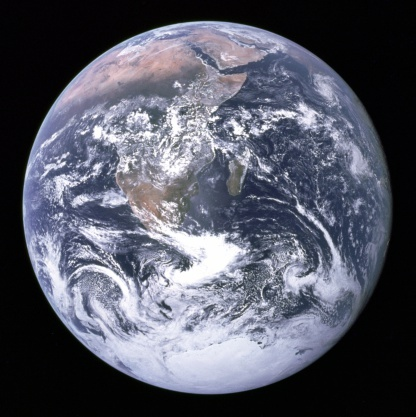
\includegraphics[width=\linewidth]{figures/dimension-blue-marble.jpg}\par
   {\footnotesize\emph{The Blue Marble}\\NASA 摄\par}}

可以这样论证: 若选定 $X$ 中一点的两个坐标, 比如令 $x=a$ 且 $y=b$, 其中 $a,b\in K$, 那么由 $X$ 的定义方程可知, 第三个坐标受这两个选择的约束, 必须满足
\[
  z^{2}=1-a^{2}-b^{2}.
\]
特别地, 第三个坐标至多有两个可能的解.

换句话说, 要描述 $X$ 上的一个点, 有两个可以自由取值的变量: 可以不受约束地选择 $x$ 和 $y$ 坐标, 而第三个坐标随之只能取有限个可能的值. 这反映出一个代数事实: 元素 $[x],[y]\in K[X]$ 在 $K$ 上代数独立, 因为指定其中一个的值不会约束另一个. 而 $[x],[y],[z]$ 在 $K$ 上代数相关, 因为它们满足多项式关系
\[
  [x]^{2}+[y]^{2}+[z]^{2}-1=[x^{2}+y^{2}+z^{2}-1]=0\in K[X].
\]
\end{Example}

上一个例子表明, 在 $X$ 中\textquotedbl{}移动的自由度\textquotedbl{}可以用代数独立的函数来度量: 只要 $K[X]$ 中有代数独立的坐标函数, 就可以不受约束地选择这些坐标的值. 由于维数应当度量我们所能具有的最大移动自由度, 便得到以下想法.

\begin{BookKeyIdea}{仿射簇的维数}\leavevmode\label{idea:dimension-as-algebraic-independence}
仿射簇 $X$ 的维数应当等于 $K[X]$ 中在 $K$ 上代数独立的元素的最大个数.
\end{BookKeyIdea}

其实, 可以用这个想法定义维数. 我们不这样做, 是因为这个定义不太便于使用. 首先, 按这种描述甚至不清楚维数是否有限: 给定仿射簇 $X$, 如何知道 $K[X]$ 中不可能找到越来越大的代数独立函数集? 要证明这种情形不可能发生, 得先做一些准备. 第~\ref{sec:function-fields}--\ref{sec:transcendence-degree}~节将仔细完成这些准备. 然后第~\ref{sec:dimension-of-affine-varieties}~节会给出一个更便于使用的维数定义, 并证明它与上面的描述等价 (Corollary~\ref{cor:dimension-and-algebraic-independence}).

先把 Key Idea~\ref{idea:dimension-as-algebraic-independence} 作为动机记在心里, 转而讨论我们希望维数具备什么性质. 仿射簇的维数应当满足哪些基本性质? 我们先列出这些性质, 称之为维数公理.

\begin{Definition}{仿射簇的维数公理}\leavevmode\label{def:axioms-for-dimension}
如果函数
\[
  D:\left\{\text{非空仿射簇的同构类}\right\}\longrightarrow\mathbb{N}
\]
满足下列性质, 则称它为\emph{维数函数}:
\begin{enumerate}
  \item\label{ax:dimension-of-a-point} 若 $X$ 只含一个点, 则 $D(X)=0$;
  \item\label{ax:dimension-of-a-finite-union} $D(X_{1}\cup\cdots\cup X_{n})=\max\{D(X_{1}),\ldots,D(X_{n})\}$;
  \item\label{ax:dimension-of-a-hypersurface-section} 若 $X\subseteq\mathbb{A}^{n}$ 不可约, 且 $f\in K[x_{1},\ldots,x_{n}]$ 使得 $X\cap\mathcal{V}(f)$ 非空且不等于整个 $X$, 则 $D(X\cap\mathcal{V}(f))=D(X)-1$.
\end{enumerate}
\end{Definition}

简要解释一下这些维数公理. 首先, 两个同构的仿射簇具有相同的本质性质, 所以可以预期它们的维数相同. 这就是为什么我们把维数看成定义在仿射簇同构类集合上的函数. 由直观也不难看出为何要求公理~\ref{ax:dimension-of-a-point}: 在单个点上没有移动的自由, 所以一个点的维数应为零.

关于公理~\ref{ax:dimension-of-a-finite-union}, 以 $\mathbb{A}^{3}$ 中一条直线 $L$ 和一个平面 $P$ 的并为例. 如果直线包含在平面内, 它们的并就是这个平面, 因此 $\dim(L\cup P)=\dim(P)$, 即两个维数中的较大者. 然而, 如果直线不包含在平面内, \textquotedbl{}移动的自由度\textquotedbl{}这一直观想法就失效了: 在 $L\cup P$ 中能往多少个方向移动, 取决于站在哪一点. 为消除这种歧义, 我们规定取两者中较大的维数. 更一般地说, 我们会发现只有在不可约簇上才容易定义维数, 而可约簇的维数将定义为其不可约分支的维数的最大值.

最后来看公理~\ref{ax:dimension-of-a-hypersurface-section}. 将 $X$ 写成零点集 $\mathcal{V}(f_{1},\ldots,f_{m})$, 就能进一步分析这一陈述. 此时
\[
  X\cap\mathcal{V}(f)=\mathcal{V}(f_{1},\ldots,f_{m},f).
\]
换句话说, 公理~\ref{ax:dimension-of-a-hypersurface-section} 的实质是: 若再加上一个方程, 维数恰好降低一. 这个维数性质在代数几何中的重要性怎么强调都不为过. 因此, 本书称这一性质为\emph{维数论基本定理}.

\begin{BookFlowNote}[l]{%
公理~\ref{ax:dimension-of-a-hypersurface-section} 的所有假设都是必要的. 假设 $X$ 不可约, 是因为否则 $X$ 可能由两个相同维数的不可约分支组成, 而与 $\mathcal{V}(f)$ 相交时可能只选出其中一个分支.
}
\noindent 在向量空间的情形, 公理~\ref{ax:dimension-of-a-hypersurface-section} 是秩--零度定理的推论 (见 Exercise~\ref{ex:dimension-axiom-vector-space-analogue}).

例如, 在 $\mathbb{A}^{2}$ 中, 一维簇 $X=\mathcal{V}(xy)$ 是两个坐标轴的并. 与 $\mathcal{V}(x)$ 相交, 只选出一维的 $y$ 轴, 有违公理~\ref{ax:dimension-of-a-hypersurface-section} 的结论. 我们假设 $X\cap\mathcal{V}(f)$ 非空, 是因为 $\varnothing$ 没有定义维数. 我们还假设 $X\cap\mathcal{V}(f)\neq X$, 因为如果两者相等, 公理~\ref{ax:dimension-of-a-hypersurface-section} 的结论就不成立.
\end{BookFlowNote}

人们自然会问, 为什么不为维数再加几条公理. 例如, 我们或许会自然地假定 $\mathbb{A}^{n}$ 的维数为 $n$; 更一般地, 由线性方程定义的仿射簇的维数应当等于它作为向量空间的维数. 我们不作更多假设, 是因为 Definition~\ref{def:axioms-for-dimension} 中为数不多的几条公理已经唯一决定了所有仿射簇的维数, 如下所述.

\begin{Proposition}{维数函数至多有一个}\leavevmode\label{prop:uniqueness-of-dimension}
若 $D_{1}$ 和 $D_{2}$ 都是维数函数, 则对所有仿射簇 $X$ 都有 $D_{1}(X)=D_{2}(X)$.
\end{Proposition}
\begin{Proof}
证明的思路见 Exercise~\ref{ex:prove-dimension-function-unique}.
\end{Proof}

根据 Proposition~\ref{prop:uniqueness-of-dimension}, 接下来的路线已经清楚了: 我们要定义一个函数
\[
  D:\left\{\text{非空仿射簇的同构类}\right\}\longrightarrow\mathbb{N},
\]
并证明它满足 Definition~\ref{def:axioms-for-dimension} 的公理~\ref{ax:dimension-of-a-point}--\ref{ax:dimension-of-a-hypersurface-section}. 接下来三节将发展定义维数所需的代数工具. 重点是进一步理解代数相关与代数独立, 并发展超越次数这个关键概念. 第~\ref{sec:dimension-of-affine-varieties}~节用超越次数严格定义维数后, 公理~\ref{ax:dimension-of-a-point} 和~\ref{ax:dimension-of-a-finite-union} 的证明将很直接. 实际上, 用 Key Idea~\ref{idea:dimension-as-algebraic-independence} 就已经能证明它们 (见 Exercise~\ref{ex:point-has-dimension-zero-by-independence}, \ref{ex:dimension-monotonic-by-independence} 和~\ref{ex:dimension-of-union-by-independence}). 相比之下, 证明公理~\ref{ax:dimension-of-a-hypersurface-section} 要复杂得多, 其中一个关键步骤用到 Noether 正规化定理. 我们将在第~\ref{sec:fundamental-theorem-of-dimension-theory}~节完成这项工作.

\BookExerciseHeading
\begin{BookExercises}
  \item\label{ex:point-has-dimension-zero-by-independence} 假设 Key Idea~\ref{idea:dimension-as-algebraic-independence}, 证明一个点的维数为零.
  \item\label{ex:affine-space-dimension-lower-bound} 假设 Key Idea~\ref{idea:dimension-as-algebraic-independence}, 证明 $\dim(\mathbb{A}^{n})\geq n$.
  \item\label{ex:dimension-monotonic-by-independence} 设 $X,Y\subseteq\mathbb{A}^{n}$ 是仿射簇, 且 $X\subseteq Y$.
  \begin{enumerate}
    \item 设 $f_{1},\ldots,f_{m}\in K[x_{1},\ldots,x_{n}]$ 是多项式, 且
    \[
      f_{1}|_{X},\ldots,f_{m}|_{X}\in K[X]
    \]
    在 $K$ 上代数独立. 证明
    \[
      f_{1}|_{Y},\ldots,f_{m}|_{Y}\in K[Y]
    \]
    在 $K$ 上代数独立.
    \item 假设用 Key Idea~\ref{idea:dimension-as-algebraic-independence} 得到 $\dim(X)=d_{1}$ 且 $\dim(Y)=d_{2}$. 证明 $d_{1}\leq d_{2}$.
  \end{enumerate}
  \item\label{ex:dimension-of-union-by-independence} 设 $X_{1},\ldots,X_{m}\subseteq\mathbb{A}^{n}$ 是仿射簇, 令 $X=X_{1}\cup\cdots\cup X_{m}$.
  \begin{enumerate}
    \item 设 $f_{1},\ldots,f_{\ell}\in K[x_{1},\ldots,x_{n}]$ 是多项式, 且
    \[
      f_{1}|_{X},\ldots,f_{\ell}|_{X}\in K[X]
    \]
    在 $K$ 上代数独立. 证明对某个 $i$,
    \[
      f_{1}|_{X_{i}},\ldots,f_{\ell}|_{X_{i}}\in K[X_{i}]
    \]
    在 $K$ 上代数独立.
    \item 假设用 Key Idea~\ref{idea:dimension-as-algebraic-independence} 得到 $\dim(X_{i})=d_{i}$, $i=1,\ldots,m$. 证明
    \[
      \dim(X)=\max\{d_{1},\ldots,d_{m}\}.
    \]
    (提示: 一个不等式用 (a), 另一个用上一题.)
  \end{enumerate}
  \item\label{ex:dimension-function-of-affine-space} 设 $D$ 是维数函数. 证明 $D(\mathbb{A}^{n})=n$.
  \item\label{ex:dimension-axiom-vector-space-analogue} 设 $\ell_{1},\ldots,\ell_{m}$ 是 $n$ 元齐次线性多项式, 考虑由它们的共同零点定义的线性子空间 $V\subseteq K^{n}$:
  \[
    V=\mathcal{V}(\ell_{1},\ldots,\ell_{m})\subseteq\mathbb{A}^{n}=K^{n}.
  \]
  \begin{enumerate}
    \item 将 $V$ 解释成某个具体矩阵 $M$ 的核, 并用秩--零度定理将 $V$ 的维数表示成 $n$ 和 $\operatorname{rk}(M)$ 的函数.
    \item 设 $\ell$ 是另一个齐次线性方程, 考虑子空间
    \[
      W=V\cap\mathcal{V}(\ell).
    \]
    将 $W$ 解释成某个具体矩阵 $M'$ 的核. $M$ 和 $M'$ 有何关系?
    \item 利用 $M$ 和 $M'$ 的关系, 说明 $V$ 和 $W$ 的维数有何关系. 这与 Definition~\ref{def:axioms-for-dimension} 中的公理~\ref{ax:dimension-of-a-hypersurface-section} 相比如何?
  \end{enumerate}
  (提示: (c) 要考虑两种可能的情形. 是哪两种?)
  \item\label{ex:proper-nonempty-hypersurface-section} 设 $X\subseteq\mathbb{A}^{n}$ 是不只含一个点的不可约仿射簇. 证明存在 $f\in K[x_{1},\ldots,x_{n}]$ 使得
  \[
    \varnothing\subsetneq X\cap\mathcal{V}(f)\subsetneq X.
  \]
  (本题有助于做下一题.)
  \item\label{ex:prove-dimension-function-unique} 设 $D_{1}$ 和 $D_{2}$ 是维数函数.
  \begin{enumerate}
    \item 证明 $D_{1}(X)=0$ 当且仅当 $X$ 是有限个点的并, 由此得出: 只要 $D_{1}(X)=0$, 就有 $D_{1}(X)=D_{2}(X)$.
    \item 设 $m\geq1$, 并假设 $D_{1}(X)<m$ 时 $D_{1}(X)=D_{2}(X)$. 证明对所有满足 $D_{1}(X)=m$ 的 $X$, 都有 $D_{1}(X)=D_{2}(X)$.
    \item 将 (a) 和 (b) 合起来, 给出 Proposition~\ref{prop:uniqueness-of-dimension} 的归纳证明.
  \end{enumerate}
  \item\label{ex:dimension-function-need-not-exist-over-reals} 本题证明当 $K$ 不是代数闭的时, 维数函数不一定存在. 令 $K=\mathbb{R}$, 并反设存在维数函数 $D$.
  \begin{enumerate}
    \item 证明 $D(\mathbb{A}^{2})=2$ 且 $D(\{(0,0)\})=0$.
    \item 证明存在 $f$ 使得 $\{(0,0)\}=\mathcal{V}(f)\cap\mathbb{A}^{2}$.
    \item 说明 (a) 和 (b) 与 Definition~\ref{def:axioms-for-dimension} 的公理~\ref{ax:dimension-of-a-hypersurface-section} 矛盾.
  \end{enumerate}
\end{BookExercises}

\par\medskip
{\footnotesize
\noindent\textbf{开放获取.} 本章按照
\href{http://creativecommons.org/licenses/by-nc/4.0/}{Creative Commons Attribution-NonCommercial 4.0 International License}
的条款授权. 该许可允许以任何媒介或格式进行非商业性使用, 分享, 改编, 分发和复制, 但须对原作者和来源作适当署名, 提供 Creative Commons 许可的链接, 并说明是否作了修改.

\noindent
\begin{minipage}[t]{.17\linewidth}
  \vspace{0pt}
\includegraphics[width=.9\linewidth]{figures/source-cc-by-nc.png}
\end{minipage}\hfill
\begin{minipage}[t]{.81\linewidth}
  \vspace{0pt}本章的图片或其他第三方材料均纳入本章的 Creative Commons 许可, 除非材料的署名行另有注明. 如果材料未纳入本章的 Creative Commons 许可, 且您拟进行的使用未获法律规定的许可或超出允许使用的范围, 则须直接向著作权持有人取得许可.
\end{minipage}\par}
